\iffalse \bibliography{include/backmatter/magnus,include/backmatter/philip} \fi
\chapter{Introduction}
In order for organisations to remain competitive, there is a need to continuously improve time to market for new features and services. The societal transformation of moving from a product economy to a service economy has affected the way organisations deliver software \cite{mckinsey}. Cloud computing is a direct response to the need of agility and has increasingly earned the reputation of being the holy grail of application deployment \cite{7034713}. Products are required to move from business requirements to delivery as fast as possible. What allows organisations to remain competitive by managing to release new services with such agility is a new software development methodology named DevOps. The aim of DevOps is to break the wall between developers and operations professionals in order to minimize deployment delays and to streamline the delivery process \cite{Httermann:2012:DD:2380958}. New tools and new methodologies that help automate the entire release process are required in order to pursue a successful delivery process.\\

Virtual Machines (VM) and Linux Containers are popular tools that are used to simplify application release processes, especially in Cloud computing. Virtual machines permit workloads to be isolated from one another and for resource usage to be somewhat controlled \cite{vmvscontainers}. Docker, a Linux container manager, is different from running an entire virtual machine in that it delivers systems or applications packaged into containers. Instead of automating and making the deployment and management process as transparent and multi-platform as possible \cite{vmvscontainers}. Docker solves the same problem that faced the cargo industry; deliver goods in a standardized container so that any means of transport is capable of delivering the goods. A Dockerized application instance runs on a sort of lightweight VM with a complete copy of the file system, “sand-boxed” from other Dockerized instances. Each change to the file system in a container acts similarly to how revision control systems such as git works. Starting from a base image, any subsequent change is stored on a new layer which in turn decreases subsequent build times and allows for safe roll-backs.\\

When having a complete system decomposed in multiple containers, responsibilities are isolated between each other during run-time, minimizing component dependencies. This allows development teams to work independently on each container with separate versioning. This avoids the big-bang integration approach and allows the possibility to carry out A/B testing for each separated component. Docker has been strongly adopted for web-applications, such as Twitter and E-bay \cite{7034713}. Having software components containerized of course introduces some performance overhead when compared to running the application natively, as identified in \cite{7034713}. The question remains, how much overhead to performance is introduced when using Docker, especially when real-time requirements are mission critical?\\

Failing to meet the real-time requirements for autonomous self-driving vehicles could lead to a catastrophic effect. The software composed for self-driving vehicles could benefit by the use of virtualisation, during development (such as safe roll back and independent versioning) as well as post-development to ship updates and patches. In order to consider the use of visualisations for real-time systems, one needs to first understand the overhead that is introduced by virtualisation to ensure that the systems meet the real-time requirements for the safety measures needed in an autonomous self-driving vehicles.\\

\section{Background}

The engineering challenge for this research is to identify the performance overhead when utilising lightweight virtual containers as part of the deployment pipeline for real-time systems. Current literature \cite{vmvscontainers} presents results on the performance overhead when utilising Docker and KVM. However, there exists a research gap in the contexts of real-time systems and how the utilization of software containers affects the performance of such systems. The results of this study will be used to identify the overhead costs of utilizing virtual environments, such as Docker, on standard and patched operating systems (Ubuntu and Ubuntu RT-Preempt) in the context of a real time system.\\

The paper presented by C. Berger \cite{cberger} presents the exploration of a deployment strategy in the context of self-driving vehicles that utilises lightweight Docker containers. However, the paper does not look to identify the precise performance overhead when using Docker as part of the deployment strategy. This paper aims to build on the research presented by C. Berger in order to fulfil a gap in current literature by identifying such performance-costs through exploring multiple software setups, configurations and system load. Prior research paper \cite{cberger} also addresses the need for future work being done within the topic of this research.\\

Current literature \cite{vmvscontainers} presents compelling evidence for the existence of performance overhead when running applications within a virtualised environment. This evidence is based on an exploration of Docker, KVM, and native environments without exploring the impact such environments have on time critical software. This further enhances the underlying need of understanding what delay-impact virtual containers have on time critical systems such as software for self-driving vehicles. Self driving vehicles require minimal delays during runtime to allow real-time computations to enable autonomous driving that is safe. Minimal time-delay is a fundamental concern for allowing lane-following, decision making, and other computations utilized by the autonomous vehicle to interact with its surroundings.\\

While this research bases its merits on a narrow field of interest, its application can be used for a broad audience within the research community as well as for organisations interested in adopting new technology to improve software deployment for real-time systems. As more segments of today's society are becoming automated and reliant on software decision making, real-time systems plays an integral part of this development. Financial, aviation, and vehicle systems are just a few examples of domains with systems that are highly sensitive to time delays, as all of them require a time delay as close to zero as possible. A self-driving vehicle has to interpret its surroundings in real-time where any delay can have a catastrophic effect. Similarly, applications in the financial domain have to react to market fluctuations within nanoseconds to avoid loss on investment. \\

\begin{figure}[ht]
\centering
     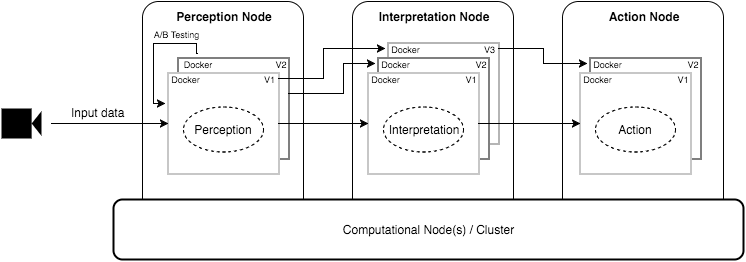
\includegraphics[width=1.0\textwidth]{./figure/containers.png}
      \caption{Run-time environment using Docker.}
       \label{containers}
\end{figure}


Figure \ref{containers} displays a deployment strategy utilising Docker in the context of self-driving vehicles. The responsibilities are broken down into three computational nodes in which Docker containers are running instances of the code base independently. Each Docker container can run different versions of the separate nodes, where the interpretation node has three versions running separately. Version one (denoted V1) in each node represents the latest working configuration while other versions are run to test code which is still under development. Aforementioned, this allows for safe and simple roll-backs in the event of buggy code or degraded performance. Furthermore, multiple versioning of the same Docker container allows for A/B testing between different containers to take place. With an always functioning configuration, the development team can demonstrate the current status to stakeholders at any point in the development cycle. The ability to demonstrate the product at any point in the development phase adds to the business value as possible investors or stakeholders can see a functioning product even though it is currently under development. With current approaches this is possible, however it is not as straight forward and easily implemented as in cases which utilizes Docker for its deployment strategy.\\

\textit{Summary: This section will provide additional information on the RT\_PREEMPT Patch, OpenDaVINCI, Operating System Schedulers, Scheduling Precision, Real Time Systems,  what is means to be a deterministic and include terminology that readers may not be familiar with.}



\section{Problem Domain \& Motivation}
Our current society is increasingly depending upon real-time systems and automated solutions for many of the fundamental building blocks to the modern world. Such systems are used within financial, aviation, and automotive sectors. Sectors where these systems play an integral role in enabling automation to provide the services we all depend on today. With these industries advancing rapidly there is a need in understanding how software engineers should best work while developing the systems that drives the progress. This research seeks to specifically answer the uncertainties that exists within the automotive industry. With work, we specifically imply the way the work flow of these software projects is structured in terms of integrating and deploying software.\\

There exists no evidence which presents argumentation how state-of-art deployment strategies impact real-time systems within autonomous self-driving vehicles and their time sensitive performance requirements. Current literature \cite{vmvscontainers} explores the overhead for general purpose operating system in the context of cloud-computing, which differs in requirements from that of an autonomous self-driving vehicle's real-time system. This creates a compelling gap in literature to explore the field of automotive by building argumentation which decision makers can rely upon when determining for which strategy is most suitable for the real-time application in question. The popularity of deployment strategies utilizing containers is steadily increasing, thus making it intriguing to understand the performance overhead introduced by containers such as Docker. While the implementation of virtualisation technologies for deployment strategies brings many advantages, there still exists uncertainty to the disadvantage of how much, if any, performance overhead they carry.\\

It is of particular importance to understand this impact for decision makers responsible for determining deployment strategies for time-critical systems utilized by self-driving vehicles. The rationale being that real-time systems are time constrained and must guarantee responses within a specified time deadline. If the system is to violate the specified deadline it may lead to software failure, which can potentially be catastrophic in the context of autonomous self-driving vehicles. Therefore it is crucial to ensure that the execution environment and deployment context will allow the real-time application to stay within its specified deadline. This is the gap in which the result of this research will seek to fulfil. Gaining specific measurement data of whether Docker carries extensive performance overhead will be an ultimate factor when deciding an approach to software deployment for real-time systems implemented in autonomous self-driving vehicles.\\

\section{Research Goal \& Research Questions}
This research seeks to understand the performance impact Docker has on real-time systems in the context of autonomous self-driving vehicles, as this context provides a solid connection to a real use case. By analysing data extracted from executions made in an application which is being implemented in vehicles today, we seek to find firm evidence which considers overhead introduced by code required for executing the real-time application (RQ1). Additional overhead may exist when executing the real-time application with other load bearing factors such as capturing images from a camera (writing and reading to disk). Thus making it important to understand how Docker affects the performance of the real-time application when including external components which are required in the development of a self-driving vehicle (RQ2).\\

\begin{enumerate}[label=\textbf{RQ\arabic*}]
\label{section:rqs}
	\item How does the respective execution environment influence the scheduling precision of the respective application?
	\item How does the respective execution environment influence the input/output performance of the respective application?\\
\end{enumerate}


\section{Contributions}
\textit{Summary: The contribution made to the research community by answering the RQs.} 


\section{Scope}
\textit{Summary: In this section we will introduce the scope which is self-driving vehicles. The hardware we are using is in-line with actual hardware used in autonomous vehicles. The software development architecture used for our experimental units have been adopted in research projects involving the actual development of autonomous vehicles. We do not aim for our results to be valid in other types of autonomous systems, such as drones. }

\section{Structure of the article}

\textit{Summary: In this section we will introduce a typical outline of the paper.}


% information on:
	% RT Preempt Patch
	% OpenDaVINCI
	% Schedulers
	% Real Time Systems
		% Time-slice
	